\chapter{Plasma Models}

	\section{\texttt{spicedmodel}: The Scalable Plasma Ion Composition and Electron Density Model}

		Python wrapper for the Scalable Plasma Ion Composition and Electron Density (SPICED) model:

		James, M. K., Yeoman, T.K., Jones, P., Sandhu, J. K., Goldstein, J. (2021), The Scalable Plasma Ion Composition and Electron Density (SPICED) model for Earth's inner magnetosphere, \emph{J. Geophys. Res. Space Physics},  \url{https://doi.org/10.1029/2021JA029565}

		\begin{figure}[h]
			\centering
			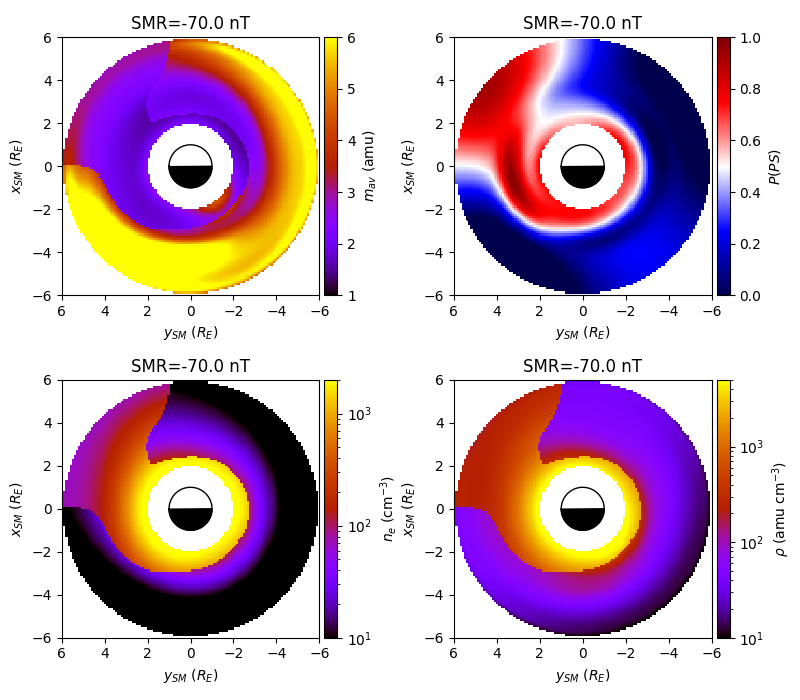
\includegraphics[width=0.9\linewidth]{figures/ch2_spicedmodel.png}
			\caption{Example output of the SPICED model.}
		\end{figure}

		\subsection{Installation}

			\subsubsection{Using \texttt{pip}}

				This will download the package from PyPI:

\begin{minted}{bash}
pip3 install spicedmodel --user
\end{minted}

			\subsubsection{From Source}

			Obtain the latest release from \url{https://github.com/mattkjames7/spicedmodel}

\begin{minted}{bash}
git clone https://github.com/mattkjames7/spicedmodel
cd spicedmodel
\end{minted}

			Either install using \texttt{setup.py}:

\begin{minted}{bash}
python3 setup.py install --user
\end{minted}

			or by building a wheel:

\begin{minted}{bash}
python3 setup.py bdist_wheel
pip3 install dist/spicedmodel-XXX.whl --user
\end{minted}

			where \texttt{"XXX"} is the rest of the file name, which will vary depending upon the current version.

			\subsection{Usage}

				Load \texttt{python3} or \texttt{ipython3}, and import

\begin{minted}{python}
import spicedmodel
\end{minted}

			\subsubsection{Accessing the models}

				There are four models, plus two additional combinations of these models:

				\begin{itemize}
					\item Plasmasphere average ion mass, $m_{\text{av,ps}}$: \texttt{spicedmodel.MavPS}
					\item Plasmatrough average ion mass, $m_{\text{av,pt}}$: \texttt{spicedmodel.MavPT}
					\item Combined average ion mass, $m_{\text{av}}$: \texttt{spicedmodel.Mav}
					\item Hot average ion mass, $m_{\text{av}}$: \texttt{spicedmodel.MavHot}
					\item Probability of being within the plasmasphere, $P$: \texttt{spicedmodel.Prob}
					\item Plasmasphere electron density, $n_{\text{e,ps}}$: \texttt{spicedmodel.PS}
					\item Plasmatrough electron density, $n_{\text{e,pt}}$: \texttt{spicedmodel.PT}
					\item Combined electron density, $n_{\text{e}}$ (a combination of plasmasphere, plasmatrough and probability models): \texttt{spicedmodel.Density}
					\item Combined plasma mass density, $\rho$: \texttt{spicedmodel.PMD}
				\end{itemize}

				The average versions of each model can be accessed simply by providing the positions in the equatorial plane where you would like them, e.g.:

\begin{minted}{python}
#either using SM x and y coordinates
P = spicedmodel.Prob(x,y)

#or using MLT (M) and L-Shell (L)
P = spicedmodel.Prob(M,L,Coord='ml')
\end{minted}

				The scaled models can be accessed using the same functions, this time including the \texttt{SMR} keyword (for \texttt{Mav}, \texttt{MavPS}, \texttt{MavPT}, \texttt{Prob}, \texttt{PS}, \texttt{PT}, \texttt{Density} or \texttt{PMD}) or \texttt{F107} (for \texttt{MavHot}), e.g.:

\begin{minted}{python}
#electron density
ne = spicedmodel.Density(x,y,SMR=-75.0)

#average ion mass
mav = spicedmodel.Mav(x,y,SMR=-75.0)

#plasma mass density, effectively ne*mav
pmd = spicedmodel.PMD(x,y,SMR=-75.0)
\end{minted}

				\subsubsection{Plotting the models}

					A simple function is included, \texttt{PlotEq}, which allows the plotting of any of the models in the equatorial plane, e.g.:

\begin{minted}{python}
ax = spicedmodel.PlotEq(ptype,SMR=-75.0)
\end{minted}

					where \texttt{ptype} is used to tell the function which model to plot, available options are: \texttt{'mav'|'mavps'|'mavpt'|'mavhot'|'prob'|'ps'|'pt'|'density'|'pmd'}.

					The following code produces a plot with all 6 models when SMR = -75 nT

\begin{minted}{python}
import matplotlib.pyplot as plt
import spicedmodel

#create the plot window
plt.figure(figsize=(8,7))

#set the parameters of the models
smr = -70.0

#plot the average ion mass
ax0 = spicedmodel.PlotEq('mav',SMR=smr,fig=plt,maps=[2,2,0,0])

#plot probability 
ax1 = spicedmodel.PlotEq('prob',SMR=smr,fig=plt,maps=[2,2,1,0])

#plot electron density 
ax4 = spicedmodel.PlotEq('density',SMR=smr,fig=plt,maps=[2,2,0,1])

#plot plasma mass density
ax5 = spicedmodel.PlotEq('pmd',SMR=smr,fig=plt,maps=[2,2,1,1])

#adjust everything to fit
plt.tight_layout()
\end{minted}


	\section{\texttt{spiced}}

		GitHub: \href{https://github.com/mattkjames7/spiced.git}{https://github.com/mattkjames7/spiced.git}

		The C++ code behind the SPICED model. It should be possible to build this library in Linux, Windows and MacOS.

		\subsection{Installation}

			In Linux and MacOS, it should eb possible to make and install the library:
			\begin{minted}{bash}
make

#optionally install globally
sudo make install
			\end{minted}

			Or in Windows:
			\begin{minted}{bash}
compile.bat
			\end{minted}

		\subsection{Usage}

			When using this library, the header file should be included, i.e.:
			\begin{minted}{cpp}
#include <spiced.h>
			\end{minted}
			and the linker flag \texttt{-lspiced} should be used during compilation.

			The models also need to be initialized at runtime using \texttt{initModels();}. \texttt{spiced.h} contains a full list of the functions which can be linked to using C and other languages like Python within the \texttt{extern "C" \{\}} section; other symbols outside this section can, such as the model objects themselves may be interacted with directly using C++.

	\section{\texttt{HermeanFLRModel}: Model of Mercury's dayside plasma mass density}

		GitHub: \href{https://github.com/mattkjames7/HermeanFLRModel.git}{https://github.com/mattkjames7/HermeanFLRModel.git}

		Estimate the dayside plasma mass density in Mercury's magnetosphere using the field line resonance (FLR) based model from \citet{James2019}.

		\subsection{Installation}

			This hasn't been placed on PyPI, so either download fromt he GitHub page and install using \texttt{pip}, or clone and build the package:
			\begin{minted}{bash}
#if you download the package
pip3 install HermeanFLRModel-x.y.z-py3-none-any.whl --user

#or clone, build and install
git clone https://github.com/mattkjames7/HermeanFLRModel.git
cd HermeanFLRModel
python3 setup.py bdist_wheel
pip3 install dist/HermeanFLRModel-x.y.z-py3-none-any.whl --user
			\end{minted}
			where \texttt{x.y.z} should be replaced with the current version number.

		\subsection{Usage}

			Import the module and create an instance of the \texttt{Model} object:
			\begin{minted}{python}
import HermeanFLRModel as hflr

model = hflr.Model(Alpha,Coord='MSM')
			\end{minted}
			where \texttt{Alpha} is the power law index which should be an integer from 0 to 6, and \texttt{Coord} sets the coordinate system to use (either MSM or MSO).

			Use the \texttt{model.Calc()} member function to work out densities:
			\begin{minted}{python}
#create input coordinate(s)
x = np.zeros(6)
y = np.array([1.0,1.2,1.4,1.6,1.8,2.0])
z = np.zeros(6)

#call model Calc() function
rho = model.Calc(x,y,z)
			\end{minted}

			Or produce a plot of the plasma mass denity for a slice through the magnetosphere, e.g.:
			\begin{minted}{python}
#select magnetic local time and alpha
MLT = 6.0
Alpha = 3.0

#plot it
ax = hflr.PlotModelSlice(MLT,Alpha)
			\end{minted}
			which should produce something like figure \ref{FigHFLR}.

			\begin{figure}
				\begin{center}
					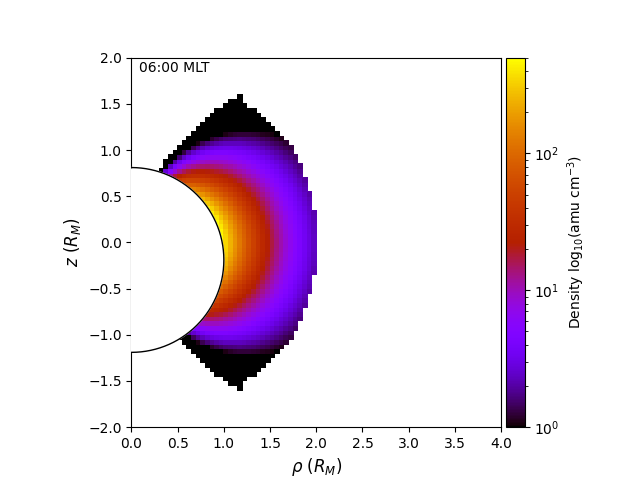
\includegraphics[width=0.8\textwidth]{figures/ch2_hflr.png}
				\end{center}
				\caption{Plasma mass density at 6:00 MLT. \label{FigHFLR}}
			\end{figure}



	\section{\texttt{PyGCPM}: Wrapper for the Global Core Plasma Model}
	
		GitHub: \href{https://github.com/mattkjames7/PyGCPM.git}{https://github.com/mattkjames7/PyGCPM.git}

		This is a Python wrapper for the Global Core Plasma Model (\citet{Gallagher2000}, \href{https://plasmasphere.nasa.gov/models/}{code found here})

		\subsection{Installation}

			This module exists on PyPI, so can be installed using \texttt{pip}:
			\begin{minted}{bash}
pip3 install PyGCPM --user
			\end{minted}

		\subsection{Usage}

			There are three functions:
			\begin{enumerate}
				\item \texttt{PyGCPM.GCPM()}: provides particle densities at positions defined in SM coordinates.
				\item \texttt{PyGCPM.PlotEqSlice()} : plots the density of a species in the equatorial plane.
				\item \texttt{PyGCPM.PlotMLTSlice()} : plots the density of a particle species in 
			\end{enumerate}

			Firstly, get some densities at some positions in SM coordinates, units of $R_E$:
			\begin{minted}{python}
import PyGCPM
ne,nH,nHe,nO = PyGCPM.GCPM(x,y,z,Date,ut,Kp=Kp,Verbose=Verbose)
			\end{minted}
			where \texttt{Date} is the date in the format yyyymmdd, \texttt{ut} is the time in hours, \texttt{Kp} is the Kp index and \texttt{Verbose=True} would display progress. The outputs of this function \texttt{ne}, \texttt{nH}, \texttt{nHe} and \texttt{nO} are the densities of electrons, protons, helium ions and oxygen ions, respectively.

			We can plot the density of a particle species in the equatorial plane:
			\begin{minted}{python}
PyGCPM.PlotEqSlice(20010902,12.0,Parameter='ne')
			\end{minted}
			which should produce the plot in figure \ref{FigPyGCPMEq}.

			\begin{figure}
				\begin{center}
					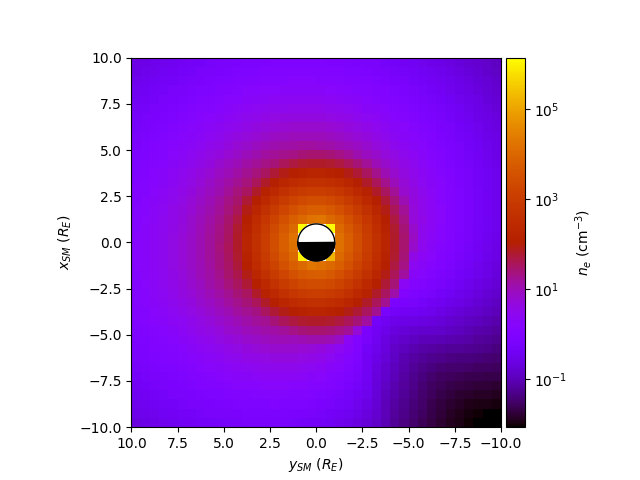
\includegraphics[width=0.8\textwidth]{figures/ch2_pygcpm_equator.png}
				\end{center}
				\caption{Equatorial electon density. \label{FigPyGCPMEq}}
			\end{figure}

			We can also plot the density of a particle species in a slice of MLT:
			\begin{minted}{python}
PyGCPM.PlotMLTSlice(8.0,20010902,12.0,Parameter='ne')
			\end{minted}
			which should produce the plot in figure \ref{FigPyGCPMMLT}.

			\begin{figure}
				\begin{center}
					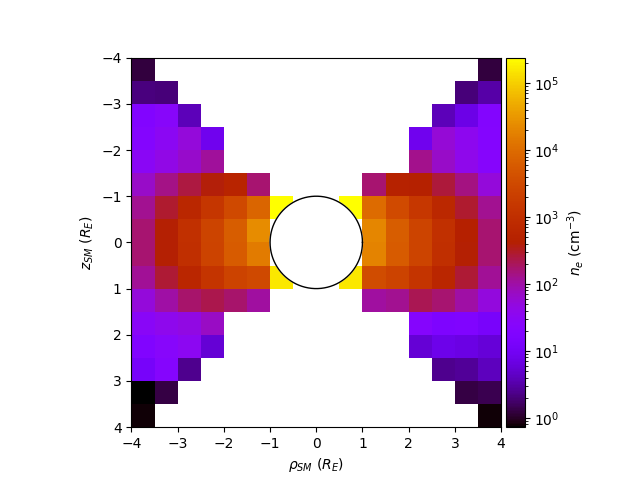
\includegraphics[width=0.8\textwidth]{figures/ch2_pygcpm_mlt.png}
				\end{center}
				\caption{MLT slice of electon density. \label{FigPyGCPMMLT}}
			\end{figure}